\section{课题主要研究内容与预期目标}

图~\ref{fig:overview} 给出了本课题三个研究内容的总体概览。

\begin{figure}[htbp]
\centering
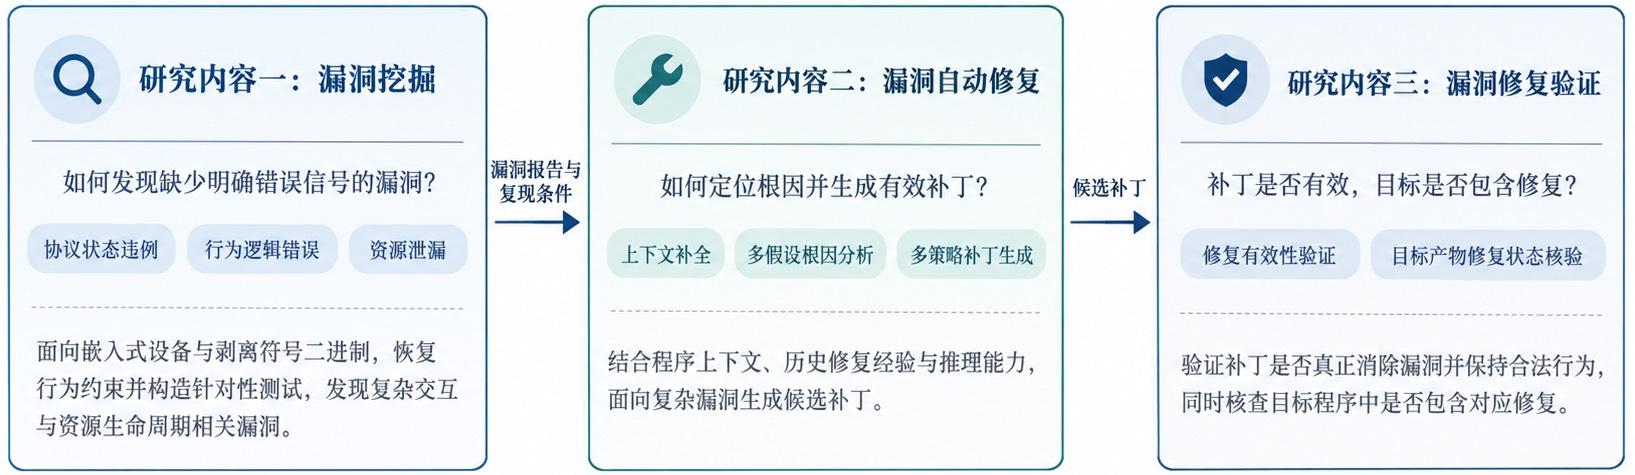
\includegraphics[width=\textwidth]{Img/overview.jpg}
\caption{研究内容总览}
\label{fig:overview}
\end{figure}

\subsection{研究目标}
\label{sec:research-objectives}

漏洞治理不仅需要发现潜在的安全缺陷，还需要针对漏洞形成有效修复，并确认修复满足相应安全要求、进入实际部署程序。仅发现漏洞或生成补丁，尚不足以确认目标系统中的相应风险已经消除。因此，本课题围绕“发现问题—生成修复—确认修复”的研究主线，探索大模型语义理解、智能体推理与程序分析相结合的方法，提升漏洞治理关键环节的自动化水平与结果可靠性。总体研究框架如图~\ref{fig:framework}~所示。

在漏洞挖掘环节，本课题重点关注嵌入式设备与剥离符号二进制场景中的协议状态违例、行为逻辑错误和资源泄漏等问题。此类问题的发现不仅需要触达相关执行路径，还需要判断程序行为是否违反协议、接口或资源生命周期要求。为此，拟研究受限信息条件下的行为约束恢复与针对性测试方法，将复杂交互中的状态变化与安全要求联系起来，提高对不易通过崩溃信号直接识别的漏洞的发现能力。

在漏洞修复环节，漏洞报告所指向的异常位置未必是实际需要修改的根因位置，而上下文缺失与过早收敛于单一解释，也可能限制修复策略的选择% TODO: 补充文献 hero（上下文缺失/过早收敛单一解释）。因此，本课题拟研究上下文增强与证据驱动的根因分析方法，结合历史修复经验开展多假设推理与多策略补丁生成，增强从漏洞表现追溯根因、从根因形成有效修改的能力，提高复杂漏洞自动修复的准确性与有效性。

在漏洞修复验证环节，补丁通过已知漏洞触发测试与功能测试，并不能充分说明漏洞根因已经消除\cite{rrbench}；同时，参考补丁的存在也不能直接证明实际部署的二进制包含对应修复\cite{zhang2026agenticppt}。为此，本课题拟从修复有效性与目标产物修复状态两个层面开展研究：一方面检查补丁是否满足漏洞相关安全要求并保持必要的合法行为，另一方面分析目标程序是否包含对应修复，提高对不完整修复、功能回归及修复缺失的识别能力。

基于上述目标，本课题形成\textbf{基于智能体的漏洞挖掘、基于智能体的漏洞自动修复、基于智能体的漏洞修复验证}三个研究内容。三者分别面向漏洞发现、候选补丁生成与修复结果确认，在任务目标上逐步衔接，共同为从漏洞识别到修复确认提供方法与技术支撑。

\begin{figure}[htbp]
\centering
\begin{tikzpicture}[node distance=0.5cm]
  % ---- 应用层 ----
  \node[smallbox, text width=2.9cm] (c1) {\textbf{内容一}\\漏洞挖掘};
  \node[smallbox, text width=2.9cm, right=1.1cm of c1] (c2) {\textbf{内容二}\\漏洞自动修复};
  \node[smallbox, text width=2.9cm, right=1.1cm of c2] (c3) {\textbf{内容三}\\漏洞修复验证};
  \draw[arr] (c1) -- node[above, font=\scriptsize]{PoC/根因} (c2);
  \draw[arr] (c2) -- node[above, font=\scriptsize]{候选补丁} (c3);
  \draw[darr] (c3.south) .. controls +(0,-0.55) and +(0,-0.55) .. node[below, font=\scriptsize]{安全规约反哺} (c1.south);
  \begin{scope}[on background layer]
    \node[layerbox, fit=(c1)(c2)(c3), label={[layerlabel]north west:应用层：漏洞攻防闭环}] (applayer) {};
  \end{scope}
  % ---- 方法层 ----
  \node[module, below=0.9cm of applayer, align=center] (method) {%
    \textbf{方法层：统一语义建模与智能体推理增强}\\
    漏洞语义表示 \quad 补丁语义表示 \quad 修复语义表示 \quad 跨环节能力迁移};
  % ---- 基础设施层 ----
  \node[module, below=0.4cm of method, align=center] (infra) {%
    \textbf{智能体基础设施层：Agent Harness 与工具链}\\
    规划—执行—反思循环 \quad 工具调用接口 \quad 上下文与记忆管理\\
    二进制分析（binutils/Ghidra）\quad 源码分析 \quad 模糊测试 \quad 符号执行};
  % ---- 数据层 ----
  \node[module, below=0.4cm of infra, align=center] (data) {%
    \textbf{数据与基准层：评估基础设施}\\
    语义漏洞基准（拟建）\quad RRBench~\cite{rrbench} \quad 561-CVE PPT 基准（已建）\cite{zhang2026pptempirical}};
\end{tikzpicture}
\caption{总体研究框架}
\label{fig:framework}
\end{figure}


\subsection{研究内容一：基于智能体的漏洞挖掘方法}

\textbf{主要研究内容}：语义/逻辑漏洞（如认证绕过、状态机错误、配置驱动缺陷）不产生崩溃信号，长期缺乏高效的自动化挖掘手段，是 IoT 与嵌入式固件安全中的突出短板。其核心难点在于：此类漏洞的触发路径通常由内部状态、配置、时序与外设响应等\textbf{自因变量}共同决定，传统输入驱动的模糊测试难以在错误的维度上有效探索；同时，语义漏洞的判定依赖人工构造的策略与规约，oracle 的缺失使自动化检测难以规模化。本研究内容旨在通过统一建模自因变量、自动构造语义 oracle、设计自因变量感知的智能体模糊测试，突破漏洞挖掘的自动化瓶颈，扩展可检测漏洞的类型与规模。

当前工作存在\textbf{自因变量难以统一建模、语义 oracle 难以自动构造}的挑战，因此，本文提出\textbf{自因变量感知的多智能体漏洞挖掘框架}。具体而言，首先综合静态分析与智能体推理，在固件二进制上识别各类自因变量，并统一表示为标注来源类型、取值空间与影响路径的自因变量格，使其成为模糊测试的一等探索维度；其次，利用智能体从协议 RFC、芯片数据手册与配置说明等自然语言文档中自动提取安全不变式，并编译为可执行的运行时监测点与断言，解决 oracle 自动构造难题；最后，设计规划—执行—验证三智能体协同的模糊测试架构，由规划智能体根据覆盖率与不变式反馈规划探索策略，执行智能体在生成输入的同时主动翻转目标自因变量（如注入中断、修改 NVRAM、模拟外设响应），验证智能体检查不变式违背并报告候选漏洞，并配套 PoC 生成与根因定位能力。

\textbf{预期目标}：构建基于智能体的漏洞挖掘系统，在真实 IoT 固件与合成基准上验证有效性，相比现有最优模糊测试方法在漏洞发现数量上提升 $\geq$ 5 倍，自因变量覆盖率 $\geq$ 70\%，安全 oracle 自动构造准确率 $\geq$ 80\%，在认证绕过、状态机错误与配置驱动缺陷三类典型漏洞上各发现若干真实漏洞并获得 CVE 编号，形成可复用的固件语义漏洞基准与工具原型。

\subsection{研究内容二：基于智能体的漏洞自动修复方法}

\textbf{主要研究内容}：漏洞自动修复是连接漏洞发现与漏洞消除的关键环节，其目标是自动定位漏洞根因、合成补丁并验证正确性。以 RRBench 为代表的大规模评估揭示了一个关键问题：现有智能体生成的"公开合理"补丁中，有相当比例（23.4\%）在私有安全性质检查下失败，且存在多个案例无法被任何系统正确修复~\cite{rrbench}。其根本原因在于：修复环节缺乏对"修复意图"的语义判定能力，智能体容易生成仅抑制特定 PoC、却未消除漏洞根因的过拟合补丁。值得注意的是，这一问题与补丁存在性测试中的"补丁语义判定"在本质上是对偶的——前者回答"生成的补丁是否构成有效修复"，后者回答"目标二进制是否包含修复"——两者均需对漏洞语义与修复语义进行深层建模。本研究内容旨在构建规约引导的可信自动修复框架，生成高质量候选补丁，并与研究内容三的修复验证方法形成"生成—验证"协同。

当前工作存在\textbf{部分规约下修复正确性难以验证、过拟合与回归难以系统抑制}的挑战，因此，本文提出\textbf{规约引导的智能体漏洞修复框架}。具体而言，首先依托统一的漏洞语义五元组表示（与研究内容一、三共享），将漏洞报告与 PoC 转化为结构化的根因语义表示；其次，借鉴 RRBench 私有 Oracle 的设计思想但将其自动化，利用智能体基于漏洞语义与代码上下文自动提取补丁必须满足的安全性质集合，既指导补丁生成又作为最终验证依据；再次，修复智能体在根因语义与安全规约的双重引导下进行多轮补丁生成与迭代，通过编译、公开测试与静态检查反馈持续修正候选补丁；最后，候选补丁交由研究内容三的修复验证环节进行 PPT 式的修复正确性判定，二者构成"生成—验证"对偶闭环，系统性抑制过拟合补丁与合法功能回归，实现部分规约下可信的自动修复。

\textbf{预期目标}：构建基于智能体的漏洞自动修复系统，在 RRBench 基准上将正确修复率从当前最优 69.6\% 提升至 $\geq$ 80\%，私有验证拒绝率降低 $\geq$ 50\%，在现有任何系统均无法正确修复的 14 个案例上成功修复 $\geq$ 4 个，形成可复用的安全规约自动提取工具链，并将方法论扩展至 C/C++ 等其他语言生态的修复基准。

\subsection{研究内容三：基于智能体的漏洞修复验证方法}

\textbf{主要研究内容}：补丁存在性测试（Patch Presence Testing，PPT）是连接漏洞披露与实际防护的关键环节，在软件供应链安全审计中具有不可替代的作用；同时，修复验证也是漏洞自动修复闭环的收官环节——自动合成的补丁是否真正消除漏洞根因，最终需要同样的补丁语义判定能力来回答。本人前期实证研究表明，前沿编码智能体已在端到端补丁存在性测试上达到与专用 SOTA 系统相当的性能~\cite{zhang2026agenticppt}，但其失败高度集中于两个环节：剥离二进制中的补丁定位，以及对后续版本中演化补丁的识别。前者源于源码级补丁意图与二进制级指令序列之间存在跨抽象层次的语义鸿沟，后者源于现有方法过度依赖补丁的形式特征而非修复意图。本研究内容旨在通过引入统一的漏洞语义表示，增强智能体在两个瓶颈环节上的推理能力，推动端到端修复状态验证从"可用"走向"可信、可扩展"，并将补丁语义判定能力对偶迁移至自动修复的补丁正确性验证。

当前工作存在\textbf{跨抽象层次补丁语义对齐困难、修复意图难以形式化}的挑战，因此，本文提出\textbf{语义先验引导的智能体修复验证增强框架}。具体而言，离线阶段利用智能体从 CVE 描述、补丁 diff 与源码上下文中提取"触发条件—危险操作—干预点—修复意图—上下文"的漏洞语义五元组，作为统一语义先验；在线阶段采用"粗—细"两阶段补丁定位，先用启发式规则快速缩小候选函数集，再以五元组为约束引导智能体在反汇编切片中进行置信度排序；针对演化补丁，提出基于修复意图的语义等价判定方法，不再追求形式上的补丁匹配，而是验证目标二进制中的干预是否实现了与原始补丁相同的安全语义。该框架在保持推理成本可控的前提下，系统性提升补丁定位准确率与演化补丁识别能力。

\textbf{预期目标}：构建基于智能体的端到端漏洞修复验证系统，在 561-CVE 基准上实现 DSR $\geq$ 0.98，在演化补丁子集上 DSR 提升 $\geq$ 15\%，在 Ubuntu 真实发行版包上保持 DSR $\geq$ 0.95，单例推理成本相比前沿配置增加不超过 10\%，形成可支撑大规模软件供应链审计与修复正确性判定的工具原型。

\subsection{预期目标与创新点}

（待撰写：分点列出理论创新、方法创新与系统/工具成果，以及预期论文与专利产出。）
